
\noindent\begin{minipage}{\textwidth}
    \begin{table}[H]
        \centering
        \caption{Hiperparâmetros e Resultados do Melhor Modelo - vgg\_v10\_BR\_opt\_aug}
        \vspace{0.2cm}
        \resizebox{\textwidth}{!}{%
            \begin{tabular}{ll | lrrr}
                \hline
                \multicolumn{2}{c|}{\textbf{Hiperparâmetros}} & \multicolumn{4}{c}{\textbf{Métricas por Classe}} \\ \hline
                \textbf{Parâmetro} & \textbf{Valor} & \textbf{Classe} & \textbf{Precisão} & \textbf{Recall} & \textbf{F1-Score} \\ \hline
    Agendador (Patience) & 3 & 31.2 & 0,5159 & 0,8784 & 0,6500 \\ 
Agendador de LR & ReduceLROnPlateau & 31.3 & 0,6310 & 0,2819 & 0,3897 \\ 
Architecture & vgg19\_bn & 31.4 & 0,5223 & 0,5658 & 0,5432 \\ 
Augmentation (Método) & None & 32.3 & 0,6344 & 0,7619 & 0,6923 \\ 
Batch Size & 32 & 32.4 & 0,9130 & 0,5833 & 0,7119 \\ 
Decaimento de Peso (WD) & 0,0017 & 33.3 & 0,7656 & 0,4537 & 0,5698 \\ 
Dropout & 0,6527 & 41.4 & 0,4286 & 0,6383 & 0,5128 \\ 
Função de Perda & CrossEntropyLoss & 41.5 & 0,7105 & 0,6279 & 0,6667 \\ 
Hidden Units & 512 & 42.4 & 0,8788 & 0,4754 & 0,6170 \\ 
Label Smoothing & 0,0000 & 44.4 & 0,8235 & 0,8750 & 0,8485 \\ 
\cline{3-6} 
Otimizador & SGD & \textbf{Média (Macro)} & 0,7014 & 0,6487 & 0,6510 \\ 
Taxa de Aprendizado (LR) & 2,44e-03 & \textbf{MCC} & \multicolumn{3}{c}{0,5732} \\ 
Unfreeze Layers & 3 &  & & &  \\ 
            \hline
            \end{tabular}%
        }
    \end{table}

    \begin{figure}[H]
        \centering
        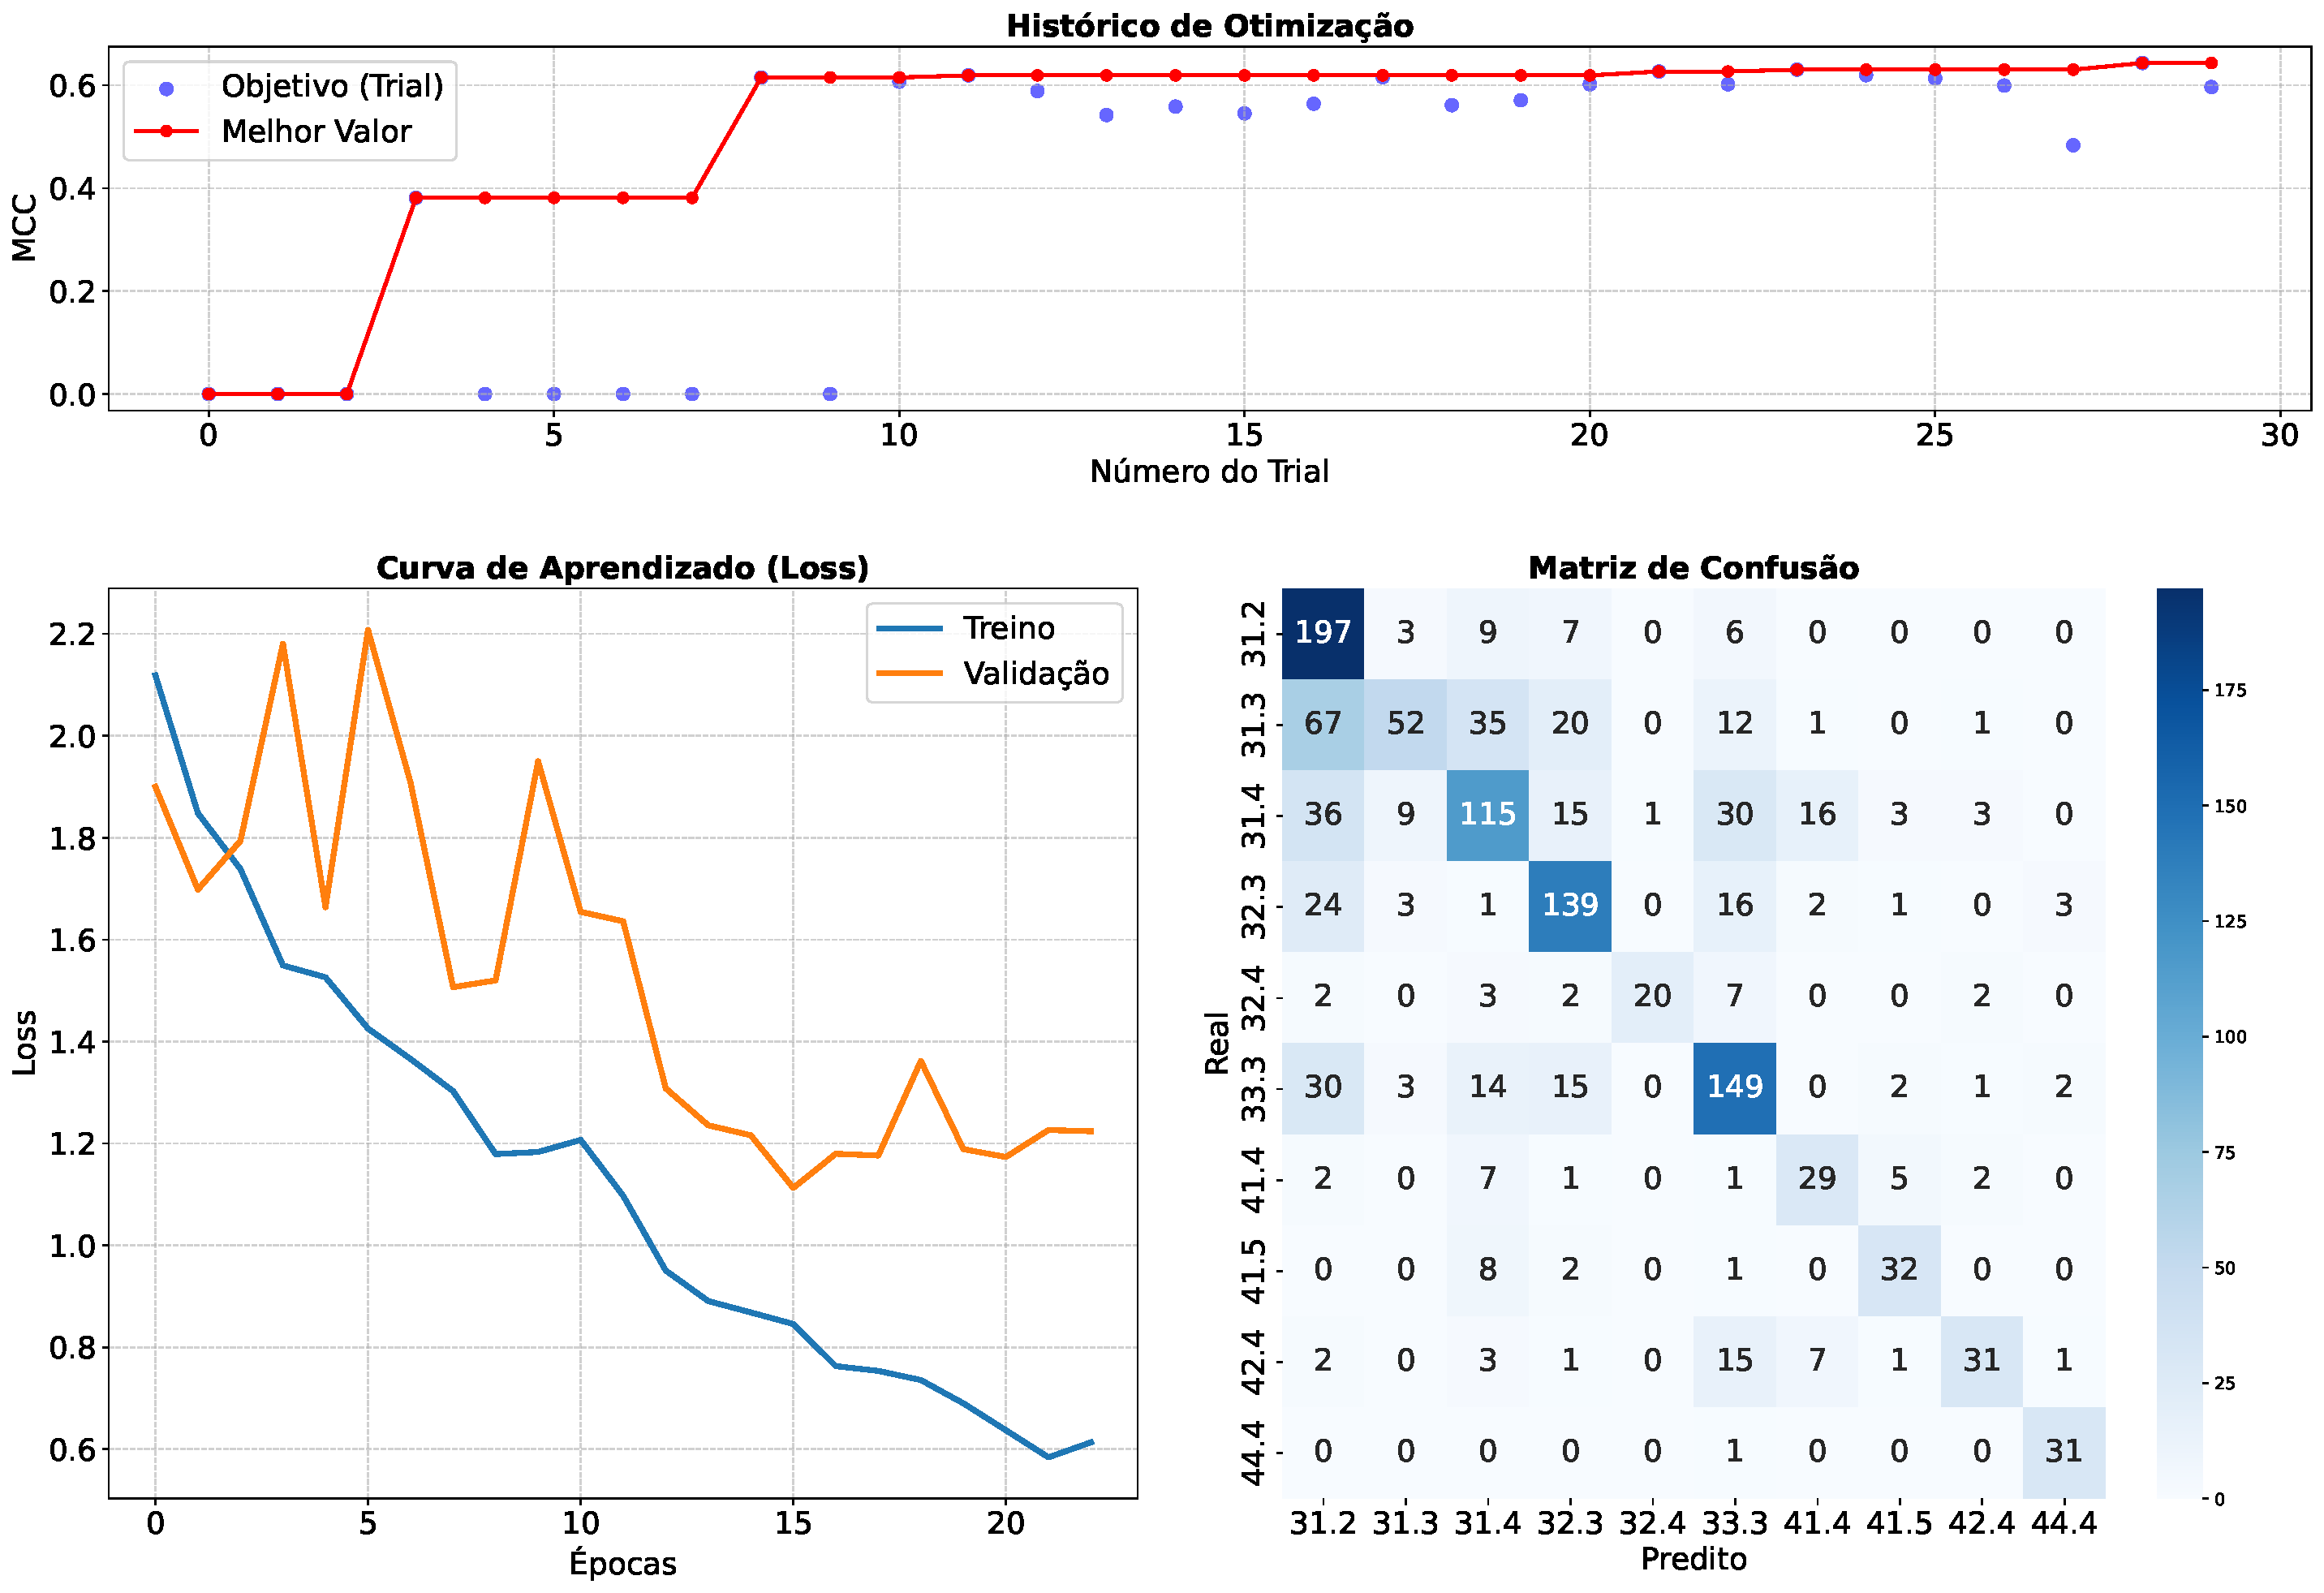
\includegraphics[width=0.85\textwidth]{tex/appendix/experiments/vgg_v10_BR_opt_aug/dashboard_consolidado.pdf}
        \caption{Histórico de Otimização, Curvas de Aprendizado e Matriz de Confusão - vgg\_v10\_BR\_opt\_aug}
    \end{figure}
\end{minipage}
\clearpage
